
\documentclass[a4paper, 12pt]{article}
\usepackage[top=3cm, bottom=3cm, left = 2cm, right = 2cm]{geometry} 
\geometry{a4paper} 
\usepackage[utf8]{inputenc}
\usepackage{textcomp}
\usepackage{graphicx} 
\usepackage{amsmath,amsthm,amsfonts,amssymb,dsfont,mathtools,blindtext} %pacotes mate
\usepackage[brazil]{babel}
\usepackage{bm}  
\usepackage[pdftex]{hyperref}
\usepackage[pdftex,bookmarks,colorlinks,breaklinks]{hyperref}  
%\hypersetup{linkcolor=black,citecolor=black,filecolor=black,urlcolor=black} % black links, for printed output
\usepackage{memhfixc} 
\usepackage{pdfsync}  

\pagestyle{fancy}
\documentclass[a4paper]{article}

\usepackage[utf8]{inputenc}    
\usepackage[brazil]{babel}
\usepackage{listings}
\usepackage{color}
 
\definecolor{dkgreen}{rgb}{0,0.6,0}
\definecolor{gray}{rgb}{0.5,0.5,0.5}
\definecolor{mauve}{rgb}{0.58,0,0.82}
 
\lstset{
  language=Python,                
  basicstyle=\footnotesize,           
  numbers=left,                   
  numberstyle=\tiny\color{gray},  
  stepnumber=2,                             
  numbersep=5pt,                  
  backgroundcolor=\color{white},    
  showspaces=false,               
  showstringspaces=false,         
  showtabs=false,                 
  frame=single,                   
  rulecolor=\color{black},        
  tabsize=2,                      
  captionpos=b,                   
  breaklines=true,                
  breakatwhitespace=false,        
  title=\lstname,                               
  keywordstyle=\color{blue},          
  commentstyle=\color{dkgreen},       
  stringstyle=\color{mauve},     
}


\begin{figure}
\flushright

\includegraphics[width=5cm]{logo-fatec.png}
\end{figure}



\title{TRABALHO DE MATEMÁTICA}


\author{Gustavo Pinho e Silva\\Matheus Henrique de Barros Ileck\\ Roberta Carioca Braz}
\vspace{3.5cm}
\date{2022}



\begin{document}
\maketitle
\pagebreak

\begin{document}
\section{Teorema de Laplace}
O teorema de Laplace consiste em escolher uma das filas (linha ou coluna) da matriz e somar os produtos dos elementos dessa fila pelos seus respectivos cofatores.


\subsection{Matriz 4x4}
\[
  A_{3\times4} =
  \left[ {\begin{array}{cccc}
    a_{11} & a_{12} & a_{13} & a_{14}\\
    a_{21} & a_{22} & a_{23} & a_{24}\\
    a_{31} & a_{32} & a_{33} & a_{34}\\
    a_{41} & a_{42} & a_{43} & a_{44}\\
  \end{array} } \right]
\]
\\
Det A = a11 . A11 + a21 . A21 + a31 . A31 + a41 . A41
\\
Aij = (-1) i+j . Dij
\\
\subsection{Exemplo de Matriz 4x4}
\begin{displaymath}
A=\begin{bmatrix}
2&-3&-1&2\\
0&-4&-3&5\\
1&2&1&3\\
0&4&1&0
\end{bmatrix} 
\end{displaymath} 
\\
2 . C_{11} + 0 . C_{21} + 1 . C_{31} + 0  .  C_{41}
\\
\\C_{11} = (-1)^1^+^1.
\left[ {\begin{array}{cccccc}
4&-3&3&|&4&-3\\
3&3&3&|&3&3\\
4&1&0&|&4&1
\end{array} } \right]
\]\\
\\
(0 + 36 + 10)  - ( 20+ 12 + 0)\\
-26 - 32\\
\textbf{-58}
\\
\\C_{31} = (-1)^3^+^1.
\left[ {\begin{array}{cccccc}
3&-1&2&|&3&-1\\
4&3&5&|&4&3\\
4&1&0&|&4&1
\end{array} } \right]
\]\\
\\
(0 - 20 + 8) - (24 + 15 + 0)\\
-12 - (-9)\\
\textbf{-3}\\
\\
Det A = 2 . 1 . (-58) + 1 . 1 . (-3) = -116 - 3 = \textbf{-119}
\pagebreak{}
\section{Determinante com Numpy e sem Numpy}
    \subsection{Código Fonte - Pyton}
        \begin{lstlisting}
#Inicio Determinante com Numpy
from numpy import matrix, linalg
import matplotlib.pyplot as plt
import time

tempo_numpy = time.perf_counter_ns()


matriz = matrix([[2,3,-1,2],
                 [0,4,-3,5],
                 [1,2,1,3],
                 [0,4,1,0]])


print("A Matriz A é: "'\n',matriz)

resultado = linalg.det (matriz)

print("\n O derteminante da matriz A é: ", round(resultado),"\n")

tempo_final = time.perf_counter_ns()
tempo_total_NP= (tempo_final - tempo_numpy)
print(f'\n O tempo de processamento do código com numpy foi de: {tempo_total_NP} nanosegundos')

print("\n ======================================== \n")

#Fim determinante com Numpy

""" 
/////////////////////////////////////////////////////////////// 
"""

#Inicio determinante sem Numpy

tempo_inicial = time.perf_counter_ns()
def remover(matriz_original,tirar_i,tirar_j):
    matriz_nova = [[int(0) for i in range(len(matriz_original)-1)] for j in range(len(matriz_original)-1)]
    ni = 0
    for i in range(len(matriz_original)):
        nj = 0
        for j in range(len(matriz_original)): 
            if j != tirar_j: 
                matriz_nova[ni][nj] = matriz_original[i][j]
                nj += 1
        if i != tirar_i: 
            ni += 1
    return matriz_nova


def determinante(matriz_original):
    if len(matriz_original) != len(matriz_original[0]): 
        print("A matriz não é quadrada!")
        return matriz_original
    resposta = 0
    if len(matriz_original) == 2: 
        resposta = (matriz_original[0][0] * matriz_original[1][1]) - (matriz_original[1][0] * matriz_original[0][1])
        return resposta
    if len(matriz_original) > 2:
        for j in range(len(matriz_original)):
            resposta += matriz_original[0][j] * (-1)**(0+j) * determinante(remover(matriz_original,0,j))
        return resposta 
    
matriz_1 = [[2,3,-1,2],
            [0,4,-3,5],
            [1,2,1,3],
            [0,4,1,0]]

for i in range(0, 4):
  for j in range(0, 4):
    print(f'[{matriz_1[i][j]:^5}]', end='')
  print()

print("\n Determinante : ",determinante(matriz_1),"\n")
#Restante do código

#Print do tempo que demorou para rodar a parte específica do código
tempo_final = time.perf_counter_ns()
tempo_total = tempo_final - tempo_inicial

print("\nTempo para excecução sem numpy foi de: ", tempo_total ,"nanosegundos", "\n")

#Fim determinante sem Numpy

Matrizes=["Matriz sem numpy" , "Matriz com Numpy"]
vl_tempo_total=[(tempo_total)*10, tempo_total_NP]

plt.stem(Matrizes, vl_tempo_total)
plt.xlabel('Tamanho da Matriz')
plt.ylabel('Tempo de execução em nanosegundo')
plt.title('Relação tempo de execução X tamanho da Matriz')

plt.show()

    \end{lstlisting}
        \pagebreak
    \subsection{Executavél}
        \begin{lstlisting}
A Matriz A é: 
 [[ 2  3 -1  2]
 [ 0  4 -3  5]
 [ 1  2  1  3]
 [ 0  4  1  0]]

 O derteminante da matriz A é:  -119 


 O tempo de processamento do código com numpy foi de: 6282175 nanosegundos

 ============================================================================= 

[  2  ][  3  ][ -1  ][  2  ]
[  0  ][  4  ][ -3  ][  5  ]
[  1  ][  2  ][  1  ][  3  ]
[  0  ][  4  ][  1  ][  0  ]

 Determinante :  -119 


Tempo para excecução sem numpy foi de:  11828287 nanosegundos 
        \end{lstlisting}
        \pagebreak    
    \subsection{Gráfico}
        \begin{figure}[!h]
            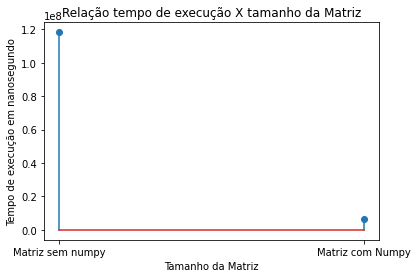
\includegraphics{Grafico1.png}
        \end{figure}
        \pagebreak
\section{Determinante das matrizes: 2x2, 3x3, 4x4, 5x5, 6x6, 7x7, 8x8, 9x9}
    \subsection{Código Fonte - Python}
        \begin{lstlisting}
        import numpy as np
import time
import matplotlib.pyplot as plt

# Entrada e Processamentos dos dados

ordem = [x for x in range(2, 10)] # lista com ordem da matriz
tempo = [] # lista para armazenar o tempo

# laço for para calcular o determinante das matriz
for x in range(2,10):
  tempo_inicial = time.perf_counter_ns()
  matriz_A = np.random.randint(10, size=(x, x)) # monta uma matriz com valores aleatorios
  determinante = np.linalg.det(matriz_A) # calcula o determinante da matriz
  tempo_final = time.perf_counter_ns()
  tempo_total = tempo_final - tempo_inicial
 # calcula o tempo total da execucao do algoritmo
  tempo.append(tempo_total)
  print(f'''Matriz = 
  {matriz_A}\n
  Determinante da Matriz de Ordem {x} = {determinante:.0f}\n 
  Tempo de execução, Matriz de Ordem {x} = {tempo_total}\n''')
print("================================================ \n")
print(f'''O tamanho das Matrizes{ordem} \n
O tempo de processamento foi de: {tempo}''')



fig, ax = plt.subplots()

grfmatriz = ['2x2', '3x3', '4x4', '5x5', '6x6', '7x7', '8x8', '9x9'] # X
counts = tempo # Y
bar_labels = 'Rosa'
bar_colors = ['tab:pink']

ax.bar(grfmatriz, counts, label=bar_labels, color=bar_colors)

ax.set_ylabel('Tempo de execução em nanosegundo')
ax.set_title('')
ax.legend(title='')

plt.show()
        \end{lstlisting}
        \pagebreak
    \subsection{Executavél}
        \begin{lstlisting}
        Matriz = 
  [[0 5]
 [5 5]]

  Determinante da Matriz de Ordem 2 = -25
 
  Tempo de execução, Matriz de Ordem 2 = 5484624

Matriz = 
  [[7 1 0]
 [3 4 6]
 [7 3 1]]

  Determinante da Matriz de Ordem 3 = -59
 
  Tempo de execução, Matriz de Ordem 3 = 230085

Matriz = 
  [[2 3 1 8]
 [6 7 8 3]
 [4 2 7 9]
 [3 8 7 8]]

  Determinante da Matriz de Ordem 4 = 1180
 
  Tempo de execução, Matriz de Ordem 4 = 129650

Matriz = 
  [[4 6 5 2 0]
 [3 6 8 1 6]
 [9 2 9 3 5]
 [5 7 6 3 3]
 [5 8 2 4 5]]

  Determinante da Matriz de Ordem 5 = 857
 
  Tempo de execução, Matriz de Ordem 5 = 110339

Matriz = 
  [[4 4 8 4 5 4]
 [1 8 6 4 5 8]
 [4 0 2 4 9 9]
 [0 8 4 3 8 8]
 [8 1 5 1 7 9]
 [3 2 0 1 8 6]]

  Determinante da Matriz de Ordem 6 = 10980
 
  Tempo de execução, Matriz de Ordem 6 = 133838

Matriz = 
  [[6 1 6 6 6 7 4]
 [3 5 4 5 4 0 7]
 [9 2 7 1 9 3 7]
 [3 4 4 4 9 9 2]
 [5 1 7 5 6 2 7]
 [2 4 7 8 4 7 7]
 [4 0 3 0 2 4 7]]

  Determinante da Matriz de Ordem 7 = -116125
 
  Tempo de execução, Matriz de Ordem 7 = 666494

Matriz = 
  [[1 3 1 7 3 6 1 0]
 [2 6 0 3 9 7 2 8]
 [9 3 8 0 7 2 6 4]
 [9 0 0 6 8 1 8 6]
 [4 9 8 7 4 2 8 8]
 [6 6 6 0 6 8 6 0]
 [0 6 7 8 4 8 0 9]
 [3 5 4 3 6 2 7 9]]

  Determinante da Matriz de Ordem 8 = -3581260
 
  Tempo de execução, Matriz de Ordem 8 = 714851

Matriz = 
  [[6 7 2 3 8 3 2 7 5]
 [0 9 6 5 4 9 2 5 0]
 [8 6 9 6 4 3 0 6 1]
 [4 2 5 4 3 6 7 3 9]
 [5 0 3 2 0 2 0 0 4]
 [2 4 7 0 3 3 9 1 9]
 [9 4 6 9 4 8 9 2 4]
 [0 9 6 9 1 6 1 1 9]
 [1 6 9 8 7 1 5 9 7]]

  Determinante da Matriz de Ordem 9 = -27315244
 
  Tempo de execução, Matriz de Ordem 9 = 141106

================================================ 

O tamanho das Matrizes[2, 3, 4, 5, 6, 7, 8, 9] 

O tempo de processamento foi de: [5484624, 230085, 129650, 110339, 133838, 666494, 714851, 141106]
        \end{lstlisting}
        \pagebreak
    \subsection{Gráfico}

        \begin{figure}[!h]
            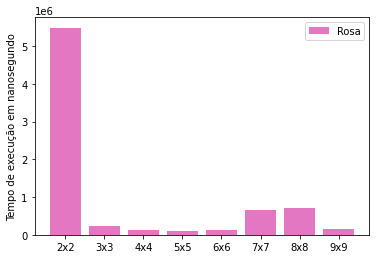
\includegraphics{Grafico2.png}
        \end{figure}
        \pagebreak
\section{GitHub}
\href{https://github.com/Gustavo-Pinho}{Gustavo Pinho e Silva}\\
\href{https://github.com/IleckMatheus}{Matheus Henrique de Barros Ileck}\\
\href{https://github.com/Ro-Cari}{Roberta Carioca Braz}
\end{document}


